%\subsection{Foundations and Examples from Strategic Management}
%\label{sub:foundations_examples}

% we introduce the reader to Dunning's framework 
The standard natural experiment resembles the
design of a randomized experiment. Naturally occurring events (such
as earthquakes \parencite[e.g.,][]{Belloc2016}) are supposed 
to determine a statistical unit's treatment status. As show in
Figure \ref{fig:ne_logic_viz}, the availability of longitudinal data
makes possible to estimate the causal effect of the treatment by
contrasting the pre-post change in the outcome variable $y$ across
the control group ($\gamma$) and the treatment group 
($ \gamma + \delta$).

\begin{figure}[]
    \centering
    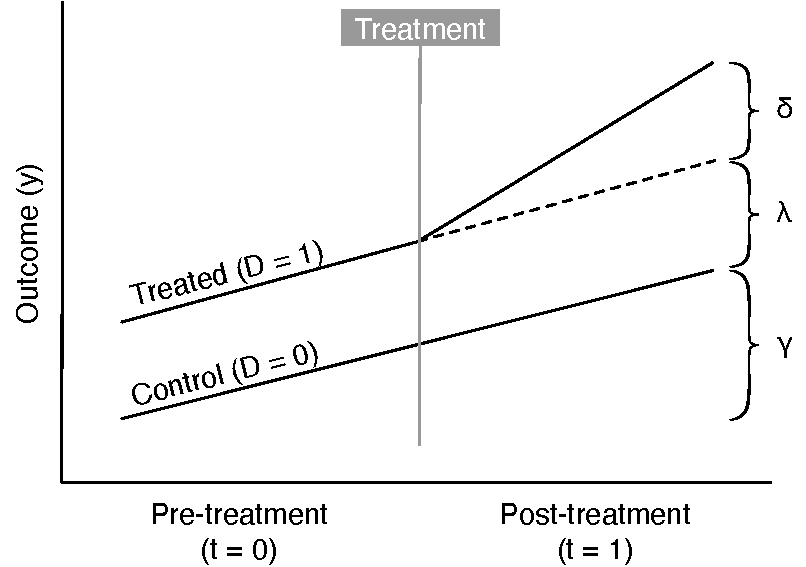
\includegraphics[width=0.75\textwidth]{exhibits/ne_logic_viz.pdf}
    \caption{Visual representation of the standard natural experiment. 
        The underlying population regression function is $y = \gamma t +
        \lambda D + \delta t D$, where $\gamma$, $\lambda$, and $\delta$ represent 
        the systematic difference in the outcome across the treated and control 
        cases, the trend effect, and the difference in the outcome that is due to
        the treatment. For the sake of clarity, we represent the case in which
        $\delta > 0$.}
    \label{fig:ne_logic_viz}
\end{figure}